\documentclass[11pt]{article}
\usepackage{ucs}
\usepackage[utf8x]{inputenc}
\usepackage{changepage}
\usepackage{graphicx}
\usepackage{amsmath}
\usepackage{gensymb}
\usepackage{amssymb}
\usepackage{enumerate}
\usepackage{tabularx}
\usepackage{lipsum}
\usepackage{hyperref}
\usepackage{fancyvrb}

\oddsidemargin 0.0in
\evensidemargin 0.0in
\textwidth 6.27in
\headheight 1.0in
\topmargin -0.1in
\headheight 0.0in
\headsep 0.0in
\textheight 9.0in

\usepackage{xcolor}

\setlength\parindent{0pt}

\newenvironment{myenv}{\begin{adjustwidth}{0.4in}{0.4in}}{\end{adjustwidth}}
\renewcommand{\abstractname}{Anotācija}
\renewcommand\refname{Atsauces}



\newcounter{alphnum}
\newenvironment{alphlist}{\begin{list}{(\Alph{alphnum})}{\usecounter{alphnum}\setlength{\leftmargin}{2.5em}} \rm}{\end{list}}


%16.3-6

\makeatletter
\let\saved@bibitem\@bibitem
\makeatother

\usepackage{bibentry}



\begin{document}
\thispagestyle{empty}


\begin{center}
{\Large C++ Exercise 8: Balanced Trees}
\end{center}

{\bf Deadline:} Monday, November 30, 2020 by 23:59:59 EET Timezone.\\ 
{\bf How to submit:} Check your code into your GitHub repository, 
the default {\tt master} branch, 
tag it as {\tt ex08submit} (all lowercase, no dashes).\\
{\bf Grading:} This exercise is worth 100\textperthousand (or $10\%$) of the total grade.\\
{\bf Objectives:} Using pointers, arrays, user-defined classes (but no external libraries like STL 
or Boost) implement an AVL tree to store string keys and
integer values.\\
{\bf Important Guideline:} The only predefined C++ libraries that can be
used during this exercise are {\tt iostream}, 
{\tt sstream}, {\tt string} (i.e. the "string" class to store 
keys and also the libraries related to input and output).\\
{\bf Another Important Guideline:} There are many AVL tree implementations in the public 
Web. You are encouraged to look at this code, but 
you should avoid any copying of large chunks of such code.
It is not just a matter of academic honesty, 
but writing your own balancing code with rotations is 
emotionally rewarding; and there may be 
subtle issues that you cannot properly address and fix unless you wrote it yourself.




\vspace{20pt}
{\bf \large Description}

In the past there have been serious concerns with hostile user behavior 
in social networks (e.g.\ the suicide of a user of 
{\em Ask.fm}, a company founded in Latvia; see \url{https://bit.ly/3lCCmZ0}). 
For this reason a highly responsible social media startup {\em InstaDraugs} 
wants to monitor all verbal abuse or 
extremist speech in user comments and posts.  
They maintain a {\em lexicon of trigger words} \textendash{}
collection of words indicating threats of violence, ethnic or racial slurs, 
sexually explicit content, swearing, verbal abuse, cyberbullying
as well as graphic descriptions of self-destructive or extremist behavior. If some 
user comment contains these words and the total badness score exceeds some threshold,
it is removed immediately or a human moderator is alerted.

{\em InstaDraugs} stores their lexicon in an 
AVL tree (an ordered Binary Search Tree satisfying the 
AVL condition) containing all sorts 
of bad words. Every word $w_i$ is associated with its badness \textendash{}
a positive integer $b_i$ (badness indicates how many instances of that word appeared
in the training datasets so far). All the entries in the lexicon look like this:
$$(w_1,b_1),\;(w_2,b_2),\;\ldots,(w_k,b_k),$$
where the keys are pairwise different. Sometimes the company finds that their lexicon
is too large; in this case they erase one or more words $w_i$
together with their associated values $b_i$. 

In addition to the {\bf insert} and {\bf erase} of words, the
lexicon also serves to {\bf find} words (i.e.\ to add up the total 
badness for some text chunk to be verified). The QA department of {\em InstaDraugs} 
also wants the ability to {\bf locate}
any given key in the lexicon (how to navigate to it from the root of the AVL tree) 
to ensure that the lexicon always operates efficiently. 
They also need the ability to {\bf dump} the entire
lexicon (or some alphabetically sorted portion of it) for further review with 
their Linguistics department.

The program starts with an empty lexicon: the underlying AVL tree contains no entries.
Every word contains one or more letters; 
{\em Instadraugs} allows $52$ letters ($26$ upper-case letters and $26$ 
lower-case letters in English alphabet). They do not analyze punctuation, 
digits or special characters to find offensive content. 
The keys in the AVL tree will never contain any hyphens, apostrophes or 
other special symbols (as well as non-English letters). 
All words are case sensitive (upper-case and lower
case letters differ; for example, \textcolor{blue}{\tt ES}, 
\textcolor{blue}{\tt es}, \textcolor{blue}{\tt Es},
and \textcolor{blue}{\tt eS} are four different words. 

There are five commands that can be
executed on this lexicon. Two of them update the map, 
the other three just read the current state of the lexicon and produce some output.
\begin{itemize}
\item {\bf Command ``insert''}, preceded
by a capital letter \textcolor{red}{\tt I}. 
It is followed by one or more
words that are inserted into a map. 
When some word (say, \textcolor{blue}{\tt abc}) is inserted for the first time, 
the map is initialized with a new entry $(\mathtt{\char`\"}\textcolor{blue}{\mathtt{abc}}\mathtt{\char`\"},1)$. 
When the same word is inserted again, 
the badness counter (its value in the map)
is incremented: the entry becomes $(\mathtt{\char`\"}\textcolor{blue}{\mathtt{abc}}\mathtt{\char`\"},2)$, 
$(\mathtt{\char`\"}\textcolor{blue}{\mathtt{abc}}\mathtt{\char`\"},3)$ and so on.
If there are multiple words on the same line, they are all inserted. 
The badness value for a word that repeats on the same line can be incremented multiple times.\\
This command always succeeds and does not produce any output.
\item {\bf Command ``erase''}, preceded
by a capital letter \textcolor{red}{\tt E}.
It is followed by one or more
words that are erased from the map. 
Such words are deleted along with their associated badness values. 
If the line with this command
contains multiple words (separated by single spaces), 
they are all erased. Erasing words that are not present in the current lexicon is ignored.\\
This command always succeeds and does not produce any output.
\item {\bf Command ``get''}, preceded by a capital letter \textcolor{red}{\tt G}.
It is followed by a {\bf single} word.\\
This command outputs the line number 
(where it is in the input file) followed 
by a space and followed by the 
entry (word and the integer value associated with it). 
If the key does not exist, the key with value $0$ should be returned
\item {\bf Command ``locate''}, preceded 
by a capital letter \textcolor{red}{\tt L}.
Such commands are followed by a {\bf single} word.\\
This command outputs the line number 
(where the line it is in the input file) 
followed by a space and the letter 
\textcolor{blue}{\tt N} (if the word was not found)
or the {\em location} of the key. The location 
can be either an asterisk \textcolor{blue}{\tt *} (if the word is the root) or 
an asterisk followed by some letters 
\textcolor{blue}{\tt L}, \textcolor{blue}{\tt R}
indicating the location of the node in the tree
(for example, \textcolor{blue}{\tt *LRR} means
that the key can be found going to the root, 
moving one step to the left and then two steps 
to the right.)
\item {\bf Command ``dump''}, preceded 
by a capital letter \textcolor{red}{\tt D}.
Such commands are followed by two arguments {\tt start} and
{\tt end}. Either of them or both can be underscores.\\
Dump command outputs its corresponding line number (from the input file) 
followed by an ordered list 
of entries in your map (all pairs $(w_i,b_i)$ 
where $w_i$ is between the start and the end (may be also equal to them).  
If the start or the end are underscores, we should dump the 
lexicon from the very beginning (or until the very end respectively).
If the {\tt end} precedes the {\tt start} (or nothing is found), 
this command returns an empty list.
\end{itemize}

\vspace{10pt}
{\bf AVL Tree}

Every insert and erase should keep the underlying 
tree as an AVL tree. 
The concrete AVL tree implementation (what types of pointers, 
classes, private/public members) is up to you, but it should
output the expected results for all the debug commands: 
If the lexicon is initialized in a certain way with insert/erase commands, 
then the location of each key has certain value (it is \textcolor{blue}{\tt *}, 
\textcolor{blue}{\tt *L}, \textcolor{blue}{\tt *R}, \textcolor{blue}{\tt *LL}, 
\textcolor{blue}{\tt *LR}, or similar). 

See (Goodrich2011, p.438--449) Chapter 10.2; all 
AVL concepts and algorithms are explained there.
See also AVL Tree Rotations reference, \url{https://bit.ly/2UEEbc8} 
(University of Florida)
and other good tutorials explaining how to manipulate AVL trees. 



\vspace{10pt}
{\bf BST Ordering}

Binary Search Trees (BSTs) rely on a certain ordering of its 
keys (in our situation \textendash{} case-sensitive words 
using the $52$-symbol English alphabet). 

The algorithm should support the following three orderings
(the specific order to use is input at the very beginning
of the algorithm). 

\vspace{5pt}
{\bf (1) Lexicographic order.} Define that word $w_1$ {\em lexicographically precedes} $w_2$ (write $w_1 \prec_{\text{lex}} w_2$), 
if $w_1$ is a prefix of $w_2$. For example $\textcolor{blue}{\mathtt{AB}} \prec_{\text{lex}} \textcolor{blue}{\mathtt{ABA}}$. 
Also define that $w_1 \prec_{\text{lex}} w_2$, if neither is a prefix of another, but 
in the first position where they differ, the symbol in $w_1$ precedes the symbol in $w_2$. 
For example, $\textcolor{blue}{\mathtt{ABBD}} \prec \textcolor{blue}{\mathtt{ABC}}$
(the 3rd letter from the start differs: $\textcolor{blue}{\mathtt{AB}}\textcolor{red}{\mathtt{B}}\textcolor{blue}{\mathtt{D}}$
and $\textcolor{blue}{\mathtt{AB}}\textcolor{red}{\mathtt{C}}$).

\vspace{5pt}
{\bf (2) Shortlex order.}  Shorter words precede longer words in the shortlex order; words of the 
same length are compared lexicographically. Namely, 
$w_1 \prec_{\text{shortlex}} w_2$ is true if and only if either $|w_1| < |w_2|$ (the length of $w_1$ is smaller; it contains
fewer letters than $w_2$) or $|w_1| = |w_2|$ and at the same time $w_1 \prec_{\text{lex}} w_2$. 

\vspace{5pt}
{\bf (3) Colexicographic order.} Define that word $w_1$ colexicographically precedes $w_2$ ($w_1 \prec_{\text{colex}} w_2$), 
if $w_1$ is a suffix of $w_2$. For example $\textcolor{blue}{\mathtt{CDE}} \prec_{\text{colex}} \textcolor{blue}{\mathtt{BCDE}}$. 
Also define that $w_1 \prec_{\text{colex}} w_2$, if neither is a suffix of another, but 
in the first position (counting from the end) where they differ, letter in $w_1$ precedes the letter in $w_2$. 
For example, $\textcolor{blue}{\mathtt{ZVYZ}} \prec_{\text{colex}} \textcolor{blue}{\mathtt{XYZ}}$
(the 3rd letter from the end differs: 
$\textcolor{blue}{\mathtt{Z}}\textcolor{red}{\mathtt{V}}\textcolor{blue}{\mathtt{YZ}}$ and 
$\textcolor{red}{\mathtt{X}}\textcolor{blue}{\mathtt{YZ}}$).


\vspace{10pt}
All the English letters are arranged alphabetically where 
different letters have {\em primary differences}. 
If two words differ only by their capitalization, then we compare their 
{\em tertiarry differences} (a capital letter
precedes the lower-case letter of the same type). Some examples: 

\begin{enumerate}
\item $\textcolor{blue}{\mathtt{abc}} \prec_{\text{lex}} \textcolor{blue}{\mathtt{ABD}}$, 
having letter $\textcolor{blue}{\mathtt{c}}$
instead of $\textcolor{blue}{\mathtt{D}}$ is a primary difference. If there is any primary 
difference between the words, the letter capitalizations (tertiary differences) are ignored.
\item $\textcolor{blue}{\mathtt{abc}} \prec_{\text{lex}} \textcolor{blue}{\mathtt{ABCA}}$; 
being a prefix of another word is also a primary difference, so the capitalization is ignored.
\item $\textcolor{blue}{\mathtt{AB}} \prec_{\text{lex}} \textcolor{blue}{\mathtt{Ab}} \prec_{\text{lex}} 
\textcolor{blue}{\mathtt{aB}} \prec_{\text{lex}} \textcolor{blue}{\mathtt{ab}}$, 
just because of the tertiary differences \textendash{} there are no 
primary differences between these words. 
(BTW, the same lexicographic order is also used in real dictionaries, see Figure~\ref{fig:oxford-dictionary}.)
\item $\textcolor{blue}{\mathtt{AbC}} \prec_{\text{shortlex}} \textcolor{blue}{\mathtt{aBC}}$: 
both words have length $3$, and there are no primary differences. But there is a tertiary 
difference: $\textcolor{blue}{\mathtt{A}}$
``slightly precedes'' the lower-case letter $\textcolor{blue}{\mathtt{a}}$, 
so  $\textcolor{red}{\mathtt{A}}\textcolor{blue}{\mathtt{bC}} 
\prec_{\text{lex}} \textcolor{red}{\mathtt{a}}\textcolor{blue}{\mathtt{BC}}$ (and for the 
words of the same length lexicographic order is same as shortlex order). 
\item $\textcolor{blue}{\mathtt{aBC}} \prec_{\text{colex}} \textcolor{blue}{\mathtt{AbC}}$
in the colexicographic order (the tertiary difference is in the 2nd position from the end: 
$\textcolor{blue}{\mathtt{a}}\textcolor{red}{\mathtt{B}}\textcolor{blue}{\mathtt{C}} < 
\textcolor{blue}{\mathtt{A}}\textcolor{red}{\mathtt{b}}\textcolor{blue}{\mathtt{C}}$). 
\item $\textcolor{blue}{\mathtt{zzz}} \prec_{\text{shortlex}} \textcolor{blue}{\mathtt{AAAA}}$, 
just because $|\textcolor{blue}{\mathtt{zzz}}| =3$ is smaller than 
$|\textcolor{blue}{\mathtt{AAAA}}|=4$, so the shortest word precedes any longer word. 
\end{enumerate}


\begin{figure}[!htb]
\center{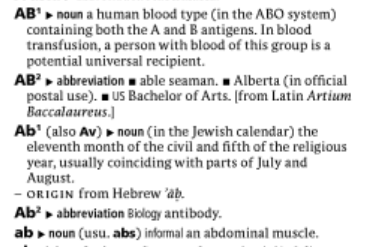
\includegraphics[width=2in]{ex08-balanced-trees/oxford-dictionary.png}}
\caption{\label{fig:oxford-dictionary} A screenshot of the 1st page of an Oxford English dictionary.}
\end{figure}

In the notation of {\tt RuleBasedCollator} (see \url{https://bit.ly/3nr0oH0}) this 
alphabetical order can be formally described like this:
$$< \textcolor{blue}{\mathtt{A}},\textcolor{blue}{\mathtt{a}} < \textcolor{blue}{\mathtt{B}},\textcolor{blue}{\mathtt{b}} < 
\textcolor{blue}{\mathtt{C}},\textcolor{blue}{\mathtt{c}} < \textcolor{blue}{\mathtt{D}},\textcolor{blue}{\mathtt{d}} < 
\ldots < \textcolor{blue}{\mathtt{W}},\textcolor{blue}{\mathtt{w}} < \textcolor{blue}{\mathtt{X}},\textcolor{blue}{\mathtt{x}} < 
\textcolor{blue}{\mathtt{Y}},\textcolor{blue}{\mathtt{y}} < \textcolor{blue}{\mathtt{Z}},\textcolor{blue}{\mathtt{z}}$$
Namely, the non-existent letter alphabetically precedes any other letter (the sequence starts with symbol $<$; shorter
words always precede any other longer words containing that shorter word).  
A pair of two letters of the same type (say, $\textcolor{blue}{\mathtt{A}},\textcolor{blue}{\mathtt{a}}$) 
can alphabetically precede another pair of letters (say, $\textcolor{blue}{\mathtt{B}},\textcolor{blue}{\mathtt{b}}$), 
but the difference between upper-case $\textcolor{blue}{\mathtt{A}}$ 
and lower-case $\textcolor{blue}{\mathtt{a}}$ is tertiary, so they are separated by a comma (not the $<$ sign).

{\em Note.} Since we are not using any accents as in French or \textcolor{blue}{\tt \"{A}}, \textcolor{blue}{\tt \"{O}}, 
\textcolor{blue}{\tt \"{U}} as in German or 
long vowels, we do not care about {\em secondary differences} between letters.\\
Some languages, including Latvian, need three levels of differences in their alphabets \textendash{} primary, secondary 
and tertiary. For example, \textcolor{blue}{\tt A} and \textcolor{blue}{\tt \=A} have a secondary difference
in most real-world dictionaries. 




\vspace{20pt}
{\bf \large Limitations}

\begin{itemize}
\item No word is longer than 30 characters. 
\item Input file can contain up to $10000$ lines
\item Input and erase commands 
contain up to $100$ words each.
\item The program should compile and run on a Linux OS (Xubuntu or similar) with 2GiB 
runtime memory; any input file should be processed into an output file under 
10 seconds and the program should exit normally (not produce a segmentation fault or 
infinite loop). 
\end{itemize}

{\em Note.} Pay some attention to your coding style, writing efficient code (in terms of 
memory use and time); and also deleting unused memory objects and avoiding 
{\em memory leaks}. These items will be discussed in our code review sessions
(and leaving them unresolved may impact the operation of {\em InstaDraugs} business, 
if they run your lexicon code for a long time and the memory leaks accumulate; in 
severe cases of memory leeks 
they need to reboot their servers and initialize their lexicon from the scratch).

For this exercise all the credit is given just for successful testcases (but the performance and
memory leak questions may arise during the code reviews that we will schedule separately).




\vspace{20pt}
{\bf \large Input}


The syntax for any input file has the first line 

\begin{verbatim}
OrderingMode
...
I wordToInsert1 wordToInsert2 ...
...
E wordToErase1 wordToErase2 ...
...
G wordToGet
...
L keyToLocate
...
D _ _
D wordBegin _
D _ wordEnd
D wordBegin wordEnd
...
F
\end{verbatim}

All input files will be valid - regarding the format and the limitations defined above. 
Explanations of the notation used in the input files:
\begin{itemize}
\item ``OrderingMode'' takes one of the following values: {\tt LEX}, 
{\tt SHORTLEX}, {\tt COLEX} (this determines the key ordering in your AVL 
tree \textendash{} it is lexicographic, shortlex or colexicographic respectively). 
If two words are equal (w.r.t. their primary differences, i.e.\ with ignore-case), then upper-case letters 
always precede the lower-case letters (see the {\em tertiary difference} defined above). 
\item ``wordToInsert1'' etc. are the words that should be inserted in the lexicon with values $1$
(or their badness should be incremented by $1$, if they already exist). 
\item ``wordToErase1'' etc. are the words that should be erased from the lexicon. 
\item ``wordToGet'' is the key for which we want to know its value (the current badness).
\item ``keyToLocate'' is the key for which we want to know its location in the AVL tree.
\item ``wordBegin'' and ''wordEnd'' are two endpoints of the interval for which we dump the entries in our lexicon. 
(either of them or both can be underscore; then the respective endpoint is not checked). 
\item {\tt F} is the marker of the end of the input; it always appears on the last line of the input. 
\end{itemize}




\vspace{20pt}
{\bf \large Output}

Commands ``insert'' and ``erase'' produce no output, but commands ``get'', ``locate'' and ``dump'' 
print the corresponding line number (where it appears in the input file) and the result of the query. 
For ``get'' it is either the entry {\tt (key,value)} or {\tt (key,0)} \textendash{} if the word {\tt key} 
was not found (and its badness is consequently $0$). 

For ``locate'' command it is the location starting
with an asterisk and letters "L" and "R". For ``dump'' it is an ordered list of entries. 


\newpage
\vspace{20pt}
{\bf \large Sample Input and Output}\\

% abate abatija abats abinieki abonements
% abatija abate abinieki abats abonements


Sample input {\bf test01in.txt}:
\begin{Verbatim}[frame=single,numbers=left]
COLEX
I abate abatija abats abats abi abinieki abonements
G abats
G abi
E abinieki abpus abra
G abinieki
L abi
L abats
L abi
D _ _
D ATE zzzzzats
D zz aa
F
\end{Verbatim}

\vspace{5pt}
Expected output {\bf test01expected.txt}:
\begin{Verbatim}[frame=single,numbers=left]
3 (abats,2)
4 (abi,1)
6 (abinieki,0)
7 *LR
8 *
9 N
10 (abatija,1) (abate,1) (abi,1) (abats,2) (abonements,1)
11 (abate,1) (abi,1) (abats,2)
12 
\end{Verbatim}

Due to the colexicographic ordering, the keys in the AVL tree should be ordered like this: 
$$\textcolor{blue}{\mathtt{abatija}} \prec_{\text{colex}} \textcolor{blue}{\mathtt{abate}} 
\prec_{\text{colex}} \textcolor{blue}{\mathtt{abi}} \prec_{\text{colex}} \textcolor{blue}{\mathtt{abinieki}}
\prec_{\text{colex}} \textcolor{blue}{\mathtt{abats}} \prec_{\text{colex}} \textcolor{blue}{\mathtt{abonements}}.$$
Looking at 3-letter suffixes makes it obvious: $\textcolor{blue}{\mathtt{ija,ate,abi,eki,ats,nts}}$
(the word ending with "a" comes first, etc.).

This order of the keys (colexicographic in this case) should be always respected 
as we build the BST. Furthermore, there are some rotation steps 
(named ``treenode restructurings'' in the textbook)
and other manipulations related to the BST insert and erase commands. 

\begin{itemize}
\item Right after {\tt abinieki} is inserted, the AVL balancing property 
is violated in the right child of the root (node {\tt abats}). We denote 
it with its child and grandchild (in the direction where the height is excessive). 
After the rotation we rearrange nodes as shown in Figure~\ref{fig:avl-trees1}. 
\item Right after {\tt abonements} is inserted, the AVL balancing property is
violated in the root itself. The rotation is shown in Figure~\ref{fig:avl-trees2}. 
\item When {\tt abi} is deleted, it is replaced by its in-order successor {\tt abats}. 
See Figure~\ref{fig:avl-trees3}.
No restructuring is needed in this case (but in other situations the AVL balance 
condition might be violated after restructuring and in these cases you should rotate). 
\end{itemize}

{\bf Note.} When deleting any internal node from a BST, there is a choice 
(and both options are technically possible as they both preserve the BST ordering invariant): 
we could take either the in-order predecessor or the in-order successor of the node you are deleting. 
In this exercise you should avoid ambiguity and always delete the in-order {\bf successor}, if there is one. 
(Otherwise the testcases will not match.)


\begin{figure}[!htb]
\center{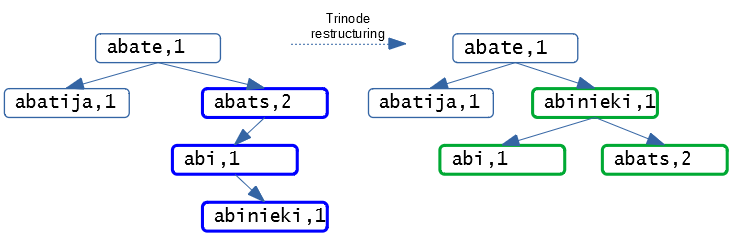
\includegraphics[width=5in]{ex08-balanced-trees/avl-trees1.png}}
\caption{\label{fig:avl-trees1} Restructuring right after inserting {\tt abinieki}.}
\end{figure}

\begin{figure}[!htb]
\center{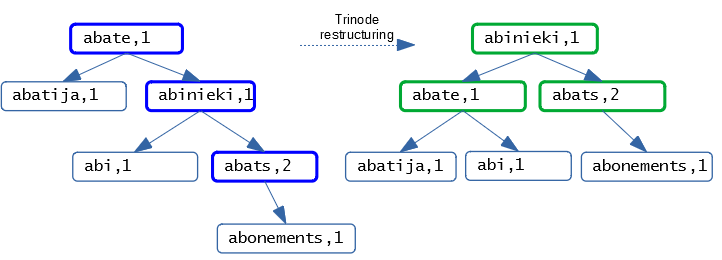
\includegraphics[width=5in]{ex08-balanced-trees/avl-trees2.png}}
\caption{\label{fig:avl-trees2} Restructuring right after inserting {\tt abonements}.}
\end{figure}

\begin{figure}[!htb]
\center{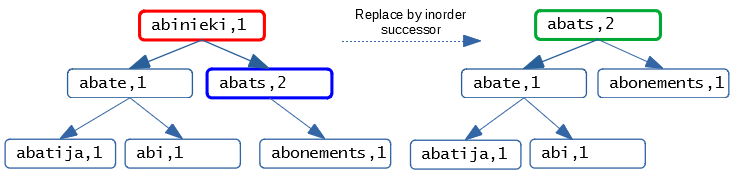
\includegraphics[width=5in]{ex08-balanced-trees/avl-trees3.png}}
\caption{\label{fig:avl-trees3} Erasing {\tt abinieki}.}
\end{figure}





\end{document}

